\documentclass[12pt]{article}
\input{bayesuvius.sty}


\begin{document}
\title{Causal DAG for genes obtained via Mappa Mundi algorithm}
\date{ \today}
\author{Robert R. Tucci\\
        tucci@ar-tiste.com}
\maketitle
\vskip2cm
\section*{Abstract}

\begin{figure}[h!]
\centering
\includegraphics[width=5in]
{two-phase-plane-bridges.png}
\caption{Suppose the two ends of bridge $a$ are equal: $\calx_1(t_a)= \calx_2(t_a')$ and
the two ends of bridge $b$ are equal too:
$\caly_1(t_b)=\caly_2(t_b')$. Also, $t_a<t_b$ and $t_a'<t_b'$. Then, there is a causal arrow pointing
from the autoregulon $\calx$ to the autoregulon 
$\caly$}
\label{fig-two-phase-plane-bridges}
\end{figure}
%\bibliographystyle{plain}
%\bibliography{references}
\end{document}